\item Consider the nonlinear control system in which it is desired to stabalize the origin
  \begin{equation}
    \dot x_1 = -2x_1 + x_2 + \sin(x_2)
  \end{equation}
  \begin{equation}
    \dot x_2 = -x_2\cos(x_1) + \cos(2x_1)u
  \end{equation}
  \begin{enumerate}
  \item verify that $(x_1, x_2, u) = (0,0,0)$ is an equilibrium. \\
    \begin{equation}
      \dot x_1 = 0 + 0 + 0 = 0
    \end{equation}
    \begin{equation}
      \dot x_2 = 0(1) + 1(0) = 0
    \end{equation}
    yes
  \item linearize the system about the origin \\
    \begin{equation}
      \dot x_1 =
      -2x_1 + x_2 =
      -2x_1 + 2x_2
    \end{equation}
    \begin{equation}
      \dot x_1 = -x_2 + u
    \end{equation}
    \begin{equation}
      \dot x =
      \begin{bmatrix}
        -2 & 1 \\
        0 & -1
      \end{bmatrix} +
      \begin{bmatrix}
        0 \\
        1
      \end{bmatrix}
    \end{equation}
  \item Study the controllability of the linearized system \\
    \begin{equation}
      \begin{bmatrix}
        B & AB
      \end{bmatrix} =
      \begin{bmatrix}
        0 & 1 \\
        1 & -1
      \end{bmatrix}
    \end{equation}
    full rank, controllable
  \item Assuming bost state variables can be measured, find a state feedback control law such that both
    eigenvalues of the linearized closed-loop system -4\\
    \begin{equation}
      \Delta_d(s) = (s+4)^2 = s^2 + 8s + 16
    \end{equation}
    \begin{equation}
      \bar \alpha = \begin{bmatrix} 8 & 16 \end{bmatrix}
    \end{equation}
    \begin{equation}
      \Delta(s) = \vert sI - A \vert =
      \begin{bmatrix}
        s+2 & -1 \\
        0 & s+1
      \end{bmatrix} = s^2 + 3s + 2
    \end{equation}
    \begin{equation}
      \alpha = \begin{bmatrix}3 & 2\end{bmatrix}
    \end{equation}
    \begin{equation}
      \bar k = \bar \alpha - \alpha = \begin{bmatrix}5 & 14\end{bmatrix}
    \end{equation}
    \begin{equation}
      Q = P^{-1} =
      \begin{bmatrix}
        0 & 1 \\
        1 & -1
      \end{bmatrix}
      \begin{bmatrix}
        1 & 3 \\
        0 & 1 
      \end{bmatrix} =
      \begin{bmatrix}
        0 & 1 \\
        1 & 2
      \end{bmatrix}
    \end{equation}
    \begin{equation}
      P = Q^{-1} = 
      \begin{bmatrix}
        0 & 1 \\
        1 & 2
      \end{bmatrix}^{-1} =
      \begin{bmatrix}
        -2 & 1 \\
        1 & 0
      \end{bmatrix}
    \end{equation}
    \begin{equation}
      k = \bar k P =
      \begin{bmatrix}5 & 14\end{bmatrix}
      \begin{bmatrix}
        -2 & 1 \\
        1 & 0
      \end{bmatrix} = 
      \begin{bmatrix}4 & 5\end{bmatrix}
    \end{equation}
    confirming:
    \begin{equation}
      A - bk =
      \begin{bmatrix}
        -2 & 1 \\
        0 & -1
      \end{bmatrix} - 
      \begin{bmatrix}
        0 \\
        1
      \end{bmatrix}
      \begin{bmatrix}4 & 5\end{bmatrix} =
      \begin{bmatrix}
        -2 & 1 \\
        0 & -1
      \end{bmatrix} - 
      \begin{bmatrix}
        0 & 0 \\
        4 & 5
      \end{bmatrix} = 
      \begin{bmatrix}
        -2 & 1 \\
        -4 & -6
      \end{bmatrix}
    \end{equation}
    eigenvalues are: $\lambda = -4, -4$
  \item Apply the state feedback control law obtained in pard d to the non=linear system above.
    Simulate and plot the state response and closed-loop system using the folowing initial conditions and
    briefly
    interpret the results:
    \begin{enumerate}
    \item $\bar x_0 = \begin{bmatrix} 1 \\ 0\end{bmatrix}$ \\
      \begin{figure}[H]
  \begin{center}
    \makebox[\textwidth]{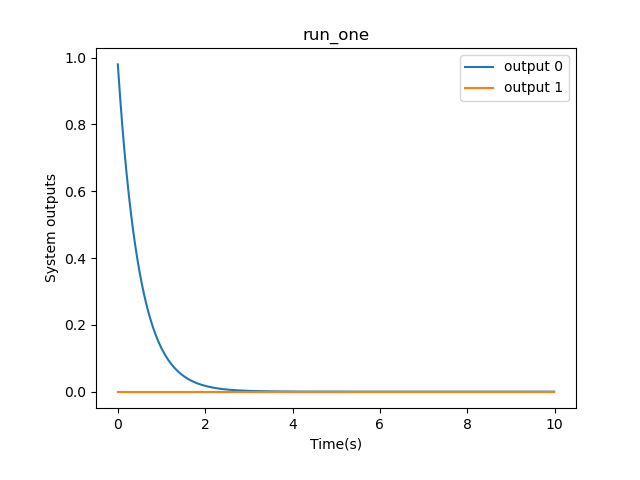
\includegraphics[max width=\textwidth]{../resources/run_one.png}}
  \end{center}
  \caption{Run One}
  \label{fig:run_one}
\end{figure}

    \item $\bar x_0 = \begin{bmatrix} 1 \\ 1\end{bmatrix}$\\
      \begin{figure}[H]
  \begin{center}
    \makebox[\textwidth]{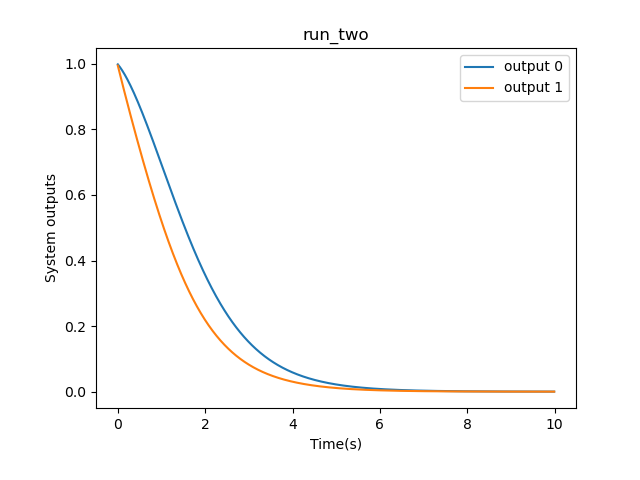
\includegraphics[max width=\textwidth]{../resources/run_two.png}}
  \end{center}
  \caption{Run Two}
  \label{fig:run_two}
\end{figure}

    \item $\bar x_0 = \begin{bmatrix} -1 \\ 1\end{bmatrix}$\\
      \begin{figure}[H]
  \begin{center}
    \makebox[\textwidth]{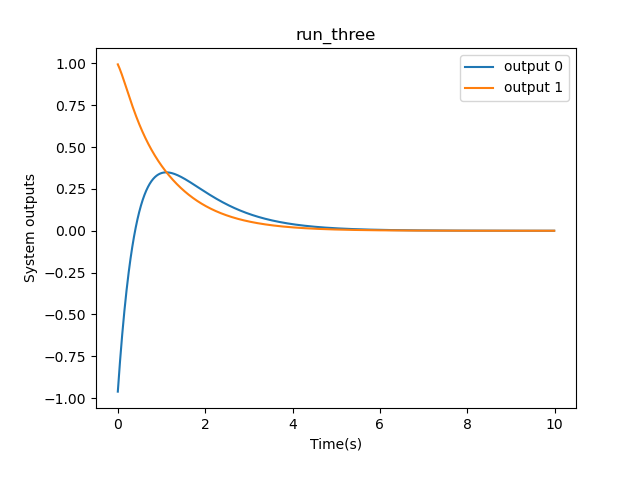
\includegraphics[max width=\textwidth]{../resources/run_three.png}}
  \end{center}
  \caption{Run Three}
  \label{fig:run_three}
\end{figure}

    \end{enumerate}
    as can be seen from \autoref{fig:run_one}, \autoref{fig:run_two}, and \autoref{fig:run_three}. The system
    takes longer to converge and has a larger overshoot the further it is from point where the linearization
    was taken.

    Just for fun, I wanted to see how the system would perform at a point much further out, and the result can
    be seen below in \autoref{fig:run_four}. As can be seen.... it can't really control the system and
    bring the outputs to 0, thus showing the limits of linearizing a non-linear system.
    \begin{figure}[H]
  \begin{center}
    \makebox[\textwidth]{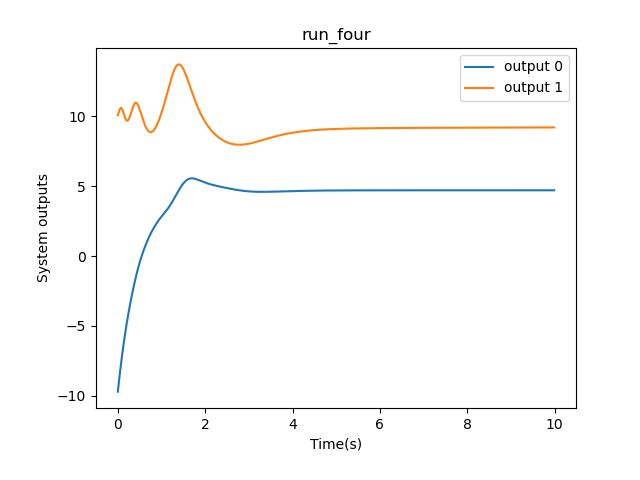
\includegraphics[max width=\textwidth]{../resources/run_four.png}}
  \end{center}
  \caption{Run Four}
  \label{fig:run_four}
\end{figure}

  \end{enumerate}